\documentclass[11pt]{report}

\usepackage[T2A]{fontenc}
\usepackage[utf8x]{inputenc}
\usepackage[english, russian]{babel}

\usepackage[T1]{fontenc}
\usepackage{titlesec, blindtext, color}
\usepackage[left=3cm, right=3cm, bottom=4cm, top=3cm, bindingoffset=0cm]{geometry}

\usepackage{amsmath}
\usepackage{mathtext}
\usepackage{environ}

\usepackage{wrapfig}
\usepackage{graphicx}
\usepackage{caption}
\usepackage{subcaption}
\usepackage{tabularx}


\graphicspath{{img/}}

\definecolor{gray75}{gray}{0.75}
\newcommand{\hsp}{\hspace{20pt}}
\addto\captionsrussian{\renewcommand{\contentsname}{Содержание}}

\titleformat{\chapter}[hang]{\Huge\bfseries}{\thechapter\hsp\textcolor{gray75}{|}\hsp}{0pt}{\Huge\bfseries}


\newenvironment{itemize*}%
  {\begin{itemize}%
    \setlength{\itemsep}{2pt}%
    \setlength{\parskip}{0.75pt}}%
  {\end{itemize}}


\newenvironment{enumerate*}%
  {\begin{enumerate}%
    \setlength{\itemsep}{2pt}%
    \setlength{\parskip}{0.75pt}}%
  {\end{enumerate}}

\newcolumntype{R}{>{\rule{0pt}{0.55cm}\raggedleft\arraybackslash}X}%
\newcolumntype{L}{>{\rule{0pt}{0.55cm}\raggedright\arraybackslash}X}%
\newcolumntype{C}{>{\rule{0pt}{0.55cm}\centering\arraybackslash}X}%
\newcolumntype{P}{>{\rule{0pt}{0.55cm}\centering\hsize=\dimexpr2\hsize+2\tabcolsep+\arrayrulewidth\relax}X}%

\newenvironment{wrapfigure*}%
 {%
  \setlength{\columnsep}{15pt}%
  \wrapfloat{figure}}%
 {\endwrapfloat}


\NewEnviron{myequation}{%
\begin{equation}
\scalebox{1.5}{$\BODY$}
\end{equation}
}



\title{
	\textbf{Escapy2.0 Engine\\Specification and User Guide}
}
\author{Генрих Тимур Домагальски}
\date{31.07.2017 Издаине 1}



\begin{document}

\maketitle

\tableofcontents

\newpage

\chapter*{О движке}
Escapy2 это игровой движок написанный на java с использованием библиотек Dagger1, libGDX и Gson. Поскольку libGDX является лишь низкоуровневой оберткой над lwjgl - движок дает полноту простора в использовании openGL, в свою очередь Dagger делает код более модульным и масштабируемым. На момент издания этого документа, движок состоит из пяти ключевых пакетов: \begin{enumerate*}
	\item Context
	\item Desktop
	\item Graphic
	\item Group
	\item Utils
\end{enumerate*}
Каждому из вышеперечисленных пакетов посвящена отдельная глава, подробнее со структурой api можно ознакомится через javadoc. На конец следует сразу заметить, что данный документ, так же как и сам движок расчитан на разработчиков неплохо знакомых с java и ООП, а так же основами openGL. Основной задачей документа не является скурпулезное описание API - за этим следует идти в javadoc, основная же цель документа - в первую очередь обрисовать возможности движка, его принцип работы, а так же life-cycle и тп.


\chapter{Начало работы}
Вход производится похожим образом как в libGDX и lwjgl - в main с созданием инстанции
\textbf{LwjglApplication}. Для этого создается объект \textbf{LwjglApplicationConfiguration} который загружается из json файла с помощью 
\textbf{EscapyDesktopConfigLoader}, о самих загрузчиках и механизме сериализации в движке более подробно потом. 
\begin{center}
	
\includegraphics[width=1.25\linewidth]{img/1.png} 
  	\label{img:12}
  	  	
  	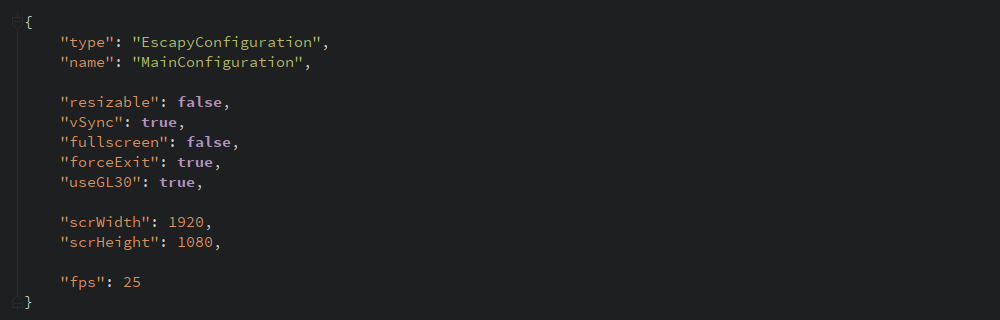
\includegraphics[width=1.25\linewidth]{img/2.png}   	
\end{center}
При создании \textbf{LwjglApplication} в качестве аргумента передается\\
\textbf{EscapyApplicationAdapter}, который в свою очередь в качестве аргумента принимает класс наследующийся от \textbf{EscapyGameContext} и varargs модулей Dagger'a.
\begin{center}
	
\includegraphics[width=1.25\linewidth]{img/3.png} 
  	\label{img:3} 
\end{center}
Подробнее о том как использовать модули Dagger'a можно прочитать на оффициальном  сайте проекта (\textit{http://square.github.io/dagger/}). \textbf{EscapyGameContext} имеет два конструктора, один из них как аргумент принимает инстанцию класса унаследованного от
\textbf{EscapyGameContextConfiguration} - абстрактного класса предоставляющего конфигурацию проекта через методы которые можно перегрузить в случае необходимости.
\begin{center}
	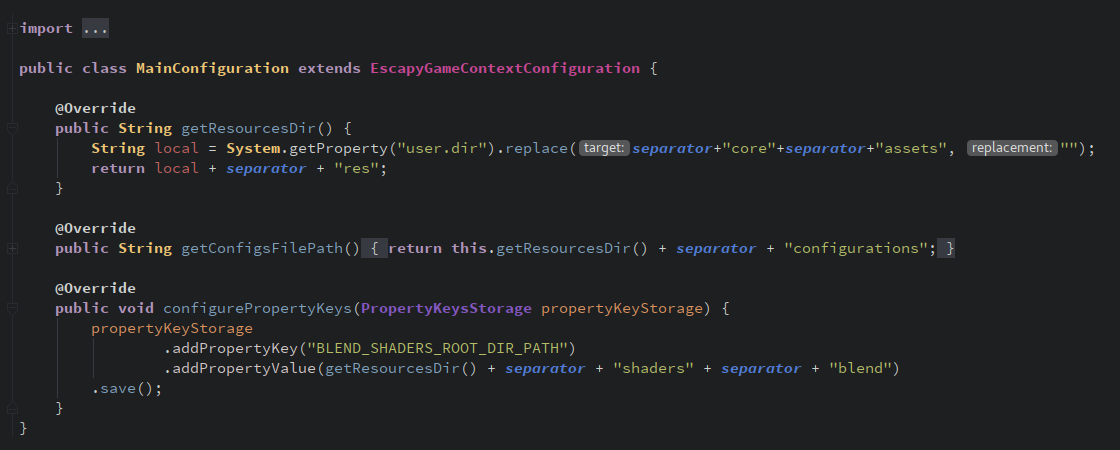
\includegraphics[width=1.2\linewidth]{img/4.png} 
  	\label{img:4} 
\end{center}


\chapter{Context}
Самый главный и значимый пакет движка в плане его архитектуры. Его основными элементами
являются два субпакета - \textit{\textbf{game}} и \textit{\textbf{annotation}} и класс
\textit{\textbf{EscapyGameContext}}. Последний наследуется от интерфейса \textit{\textbf{EscapyScreenContext}} позволяя тем самым на работу с экранами (сценами).

\section{Game}
Основные эллементы данного субпакета это классы: \begin{itemize*}
\item EscapyGameContextConfiguration - абстрактный класс делегирующий настройки
\item EscapyScreenContext - интерфейс управления экранами
\item EscapyScreen - интерфейс экрана (сцены).
\item PropertyKeysStorage - интерфейс позволяет сохранять пары ключ-объект.
\item Escapy - синглетон хранящий некоторые настройки.
\\
\end{itemize*}
\subsection*{EscapyScreen}
Отдельного внимания заслуживает этот интерфейс, он в свою очередь наследуется от интерфейса \textit{\textbf{Screen}} из библиотеки libGDX и содержит callback методы в которых должна находиться логика игры. Класс реализующий данный интерфейс, может (опционально) быть отмечен аннотацией \textit{\textbf{@SreenName("...")}}, в таком случае этому экрану будет присвоенно имя с помощью которого к этому экрану можно будет обращаться через методы интерфейса \textit{\textbf{EscapyScreenContext}}.

\section{Annotation}
Cодержит аннотации такие как \textit{\textbf{@SreenName("...")}}, а так же субпакет 
\textit{\textbf{meta}} содержащий процессор аннотаций построенный по шаблону <<Декоратор>>. Если интересуют подробности или возникло желание написать свою собственную имплементацию, то лучшем решением будет отсылка в javadoc или исходники.



\chapter{Utils}
Пакет со вспомогательными классами и прочими полезными вещами. Особого внимания заслуживают: \begin{itemize*}
	
	\item \textit{\textbf{EscapyArray и EscapyAssociatedArray}} - интерфейсы (и их 				реализации) наследующие Iterable c массивом внутри.
	
	\item Пакет \textit{\textbf{proxy}} - позволяет инстацировать объекты с listener'ами 		внутри.
	
	\item \textit{\textbf{EscapyInstanceLoader}}  - позволяет инстанцировать объекты по 		имени с помощью аннотации \textit{\textbf{@EscapyInstanced("...")}} или по имени 			метода.

	\item \textit{\textbf{EscapySerialized и EscapySimpleSerialized}} - интерфейс и 			абстрактный класс реализующий этот интерфейс, служат шаблоном для сериализуемы с помщью
	Gson'a классов.
\end{itemize*}
	\newpage
\section{EscapySimpleSerialized}
Так выглядит этот шаблон в исходниках.
\begin{center}
	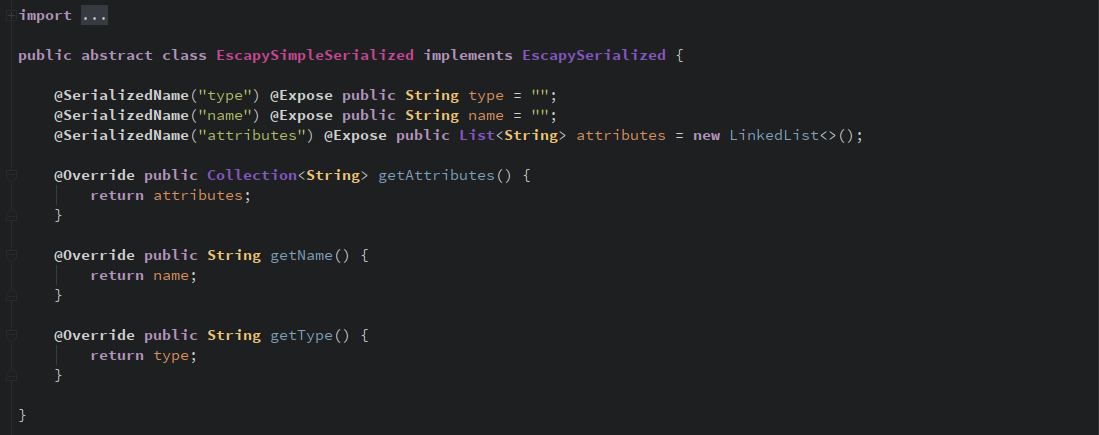
\includegraphics[width=1.2\linewidth]{img/5.png} 
  	\label{img:5} 
\end{center}	
А так выглядит его json.	
\begin{center}
	
\includegraphics[width=1.2\linewidth]{img/6.png} 
  	\label{img:6} 
\end{center}
Поскольку все классы движка должны сериализовываться через этот шаблон, код выше является необходимым минумом, для того что бы загрузчики движка могли успешно выполнить свою работу.
\newpage
\section{EscapyInstanceLoader}
Класс реализующий этот интерфейс позволяет на вызов инстанцирующих методов по имени либо самого метода, либо указанного в аннотации которым этот метод отмечен. Этот механизм очень удобен в использовании в загрузчиках движка и потому повсеместно там используется - для инстанцирования объектов по имени указаноому в json файле, либо для загрузки атрибутов для уже существующего объекта. \\Ниже пример использования - создается класс реализующий интерфейс, затем инстанция класса передается в загрузчкик.
\begin{center}
	
\includegraphics[width=1.2\linewidth]{img/7.png} 
  	\label{img:7} 
\end{center}
И в загрузчкие, во время инициализации используется для создания нужного объекта по его имени взятом из json файла.
\begin{center}
	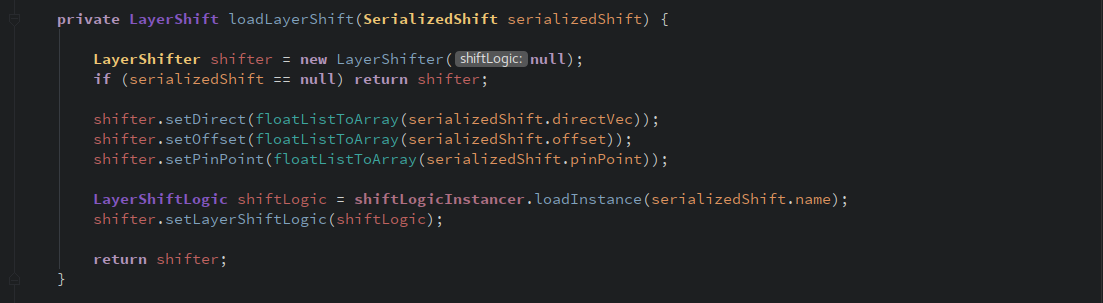
\includegraphics[width=1.2\linewidth]{img/8.png} 
  	\label{img:8} 
\end{center}

\end{document}




